

\section*{Task 3}

\subsection*{Decoder}

\begin{figure}[H]
  \begin{centering}
  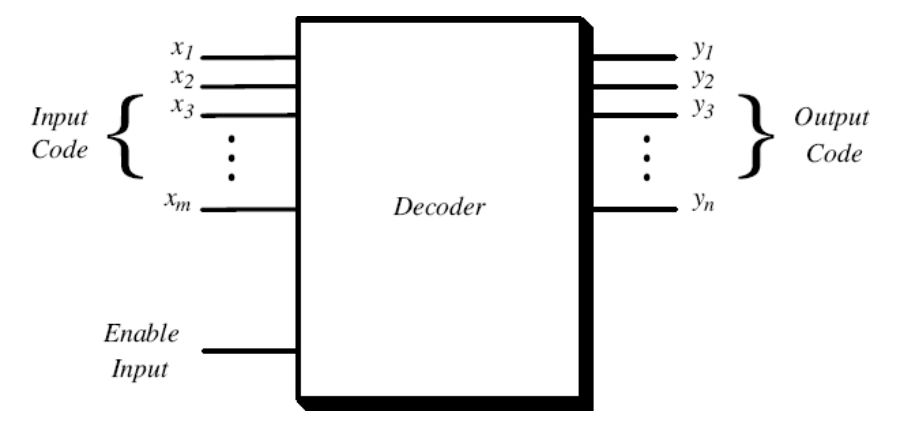
\includegraphics[scale=1]{data/decoder.png}
  \par\end{centering}
  \caption{Block Diagram of a $N:2^{N}$ Decoder}
\end{figure}


The binary decoder is a combinational logic device with N input lines and $2^{n}$ output lines, one particular combination of inputs activates one output while the remaining ones are disabled. The decoder only works when the enable input is on. Below you can find the truth table of a 2 input decoder:

\begin{figure}[H]
  \begin{centering}
  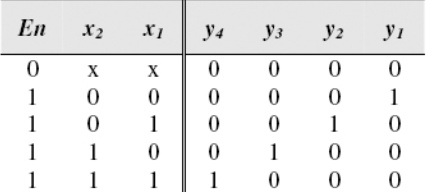
\includegraphics[scale=1]{data/decodertable.png}
  \par\end{centering}
  \caption{Truth table of a 2:4 Decoder}
\end{figure}

\subsection*{Multiplexer}

\begin{figure}[H]
  \begin{centering}
  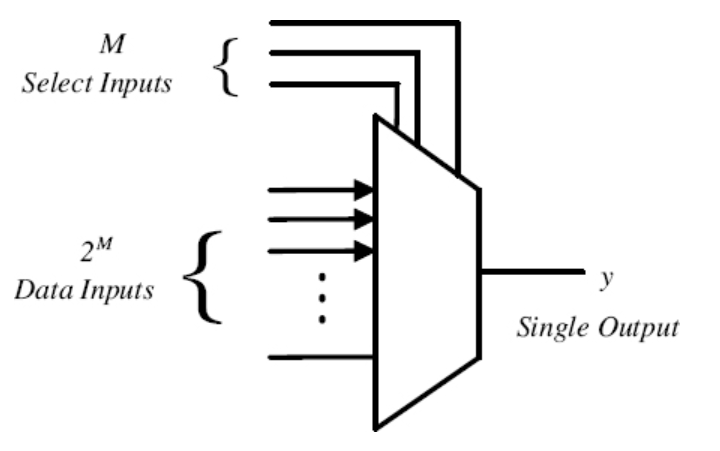
\includegraphics[scale=1]{data/muxB.png}
  \par\end{centering}
  \caption{Block Diagram of a $2^{M}:1$ Multiplexer}
\end{figure}

A multiplexer, also known as 'mux', is another combinational circuit that has $2^{M}$ inputs, M select lines and one single output. The select input lines control which data input is connected to the output. The function of a 2 input Mux is described by the truth table shown below:


\begin{figure}[H]
  \begin{centering}
  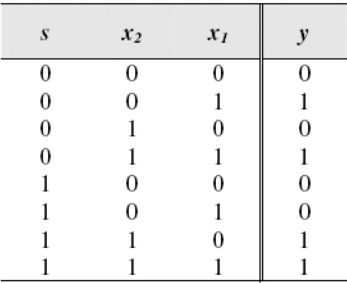
\includegraphics[scale=1]{data/muxtable.png}
  \par\end{centering}
  \caption{Truth table of a 2:1 Mux}
\end{figure}


\subsection*{About the code}

There are two different implementations of the mux and the decoder.

In one hand, both mux.v and decoder.v, use conditional statements to describe their behavior. This way is easier for the user to understand how the devices work.
Each module has it's own test bench which considers all possible inputs for a complete test.

On the other hand, newmux.v and newdecoder.v, have a variable parameter which changes the number of inputs the devices could have. The way that they are implemented is more difficult to understand than the behavioral modeling, but it is shorter. For the decoder, the shift operator resumes perfectly its function and for the mux, the index of the input array chooses the element that has to be in the output.
In order to simplify the code, instead of N input/output lines of 1 bit, it has an array of all the input's bits together. In this case the test considers all possible inputs according to parameter chosen.
  

